%%%%%%%%%%%%%%%%%%%%%%%%%%%%%%%%%%%%%%%%%%%%%%%%%%%%%%%%%%%%%%%%%%%%%%%%%%%%%%%%
%neutrino_physics.tex: Chapter on neutrino physics:
%%%%%%%%%%%%%%%%%%%%%%%%%%%%%%%%%%%%%%%%%%%%%%%%%%%%%%%%%%%%%%%%%%%%%%%%%%%%%%%%
\chapter{Theoretical Motivations}
\label{wrBosonAndHeavyNu}
%%%%%%%%%%%%%%%%%%%%%%%%%%%%%%%%%%%%%%%%%%%%%%%%%%%%%%%%%%%%%%%%%%%%%%%%%%%%%%%%
Experimental evidence \cite{NOvAresults,mainzPhaseIIResults,t2kResults} of neutrinos with non-zero masses motivates extensions to the Standard Model (SM).  
Before discussing SM extensions, the methods through which the weak bosons $W^{\pm},Z$ and fermions acquire mass 
in the SM are discussed.  Subsequently, a SM extension is presented to explain neutrino masses using the 
mass generation methods of the SM, and other experimentally observed phenomena not explained by the SM.  
The chapter concludes by presenting phenomenological aspects of this SM extension relevant to experimental 
detection.

\section{Particle Masses in the Standard Model}
\label{sec:massInSM}
The SM postulates that the four generators of the $SU(2)_{L} \times U(1)$ groups transform into the massless 
photon and massive $W^{\pm}$ and $Z$ bosons through the Brout-Englert-Higgs (BEH) mechanism.  This mechanism 
adds four degrees of freedom to the SM, in the form of a complex doublet $\Phi$ representing four bosonic 
particles, which obey the Lagrangian $\Ell_{H}$:

\begin{align}
	\Phi &= \begin{bmatrix}
	\phi^{+} \\
	\phi^{0}
	\end{bmatrix}
\end{align}

\begin{equation}
	\Ell_{H} = (D_{\mu}\Phi)^{\dagger}D^{\mu}\Phi - V(\Phi)
\end{equation}

where $V(\Phi) = \frac{1}{2}(|\Phi|^{2} - \frac{\nu^{2}}{2})$ is the Higgs potential, and 
$D_{\mu} = \partial_{\mu} + ig_{L}\tau^{j}A^{j}_{\mu} + i\frac{g'}{2}YB_{\mu}$ describes the propagation 
of the Higgs doublet $\Phi$ and its couplings to the $SU(2)_L$ generators $\tau^{j}$ and massless vector 
fields $A^{j}_{\mu}$, and the $U(1)$ generator $Y$ and massless vector field $B_{\mu}$.  $g_{L}$ and 
$g'$ determine the weak and electromagnetic interaction coupling strengths.  The Higgs doublet $\Phi$ takes a 
value $<\Phi> =$ (0  $\nu/\sqrt{2}$) so that the Higgs potential is minimized.  When $V(\Phi)$ is minimized 
and explicit matrices and values are plugged in for the group generators, the subset 
of the Lagrangian $\Ell_{H}$ without partial derivatives $\partial_{\mu}$ and the Higgs potential $V(\Phi)$:

\begin{equation}
	\Ell_{HK} = [(ig_{L}\tau^{j}A^{j}_{\mu} + i\frac{g'}{2}YB_{\mu})\Phi]^{\dagger}(ig_{L}\tau^{j}A^{j\mu} + i\frac{g'}{2}YB^{\mu})\Phi
\end{equation}

reduces to:

\begin{equation}
	\Ell_{HK} = \frac{\nu^{2}}{8}[g^{2}_{L}(A^{1}_{\mu} + iA^{2}_{\mu})(A^{1\mu} - iA^{2\mu}) + (g'B_{\mu} - g_{L}A^{3}_{\mu})^{2}]
\end{equation}

Defining the photon vector field $A_{\mu}$, and weak boson vector fields $W^{\pm}_{\mu}$ and $Z_{\mu}$ as:

\begin{equation}
	W^{\pm}_{\mu} \equiv \frac{1}{\sqrt{2}}(A^{1}_{\mu} \pm iA^{2}_{\mu}), 
	Z_{\mu} \equiv \frac{1}{\sqrt{g'^{2} + g^{2}_{L}}}(g'B_{\mu} - g_{L}A^{3}_{\mu}), 
	A_{\mu} \equiv \frac{1}{\sqrt{g'^{2} + g^{2}_{L}}}(g_{L}B_{\mu} + g'A^{3}_{\mu})
\end{equation}

yields the Lagrangian:

\begin{equation}
	\Ell_{HK} = (\frac{\nu g_{L}}{2})^{2}W^{+}_{\mu}W^{-\mu} + \frac{1}{2}(\frac{\nu \bar{g}}{2})^{2}Z_{\mu}Z^{\mu} + 0A_{\mu}A^{\mu}
\end{equation}

where $\bar{g} \equiv \sqrt{g'^{2} + g^{2}_{L}}$.  Following from this Lagrangian, the photon $A_{\mu}$ is massless, 
the $Z$ boson has mass $m_{Z} = \nu\bar{g}/2$, and the $W^{\pm}$ bosons have mass $m_{W} = \nu g_{L}/2$.  
Three of the four scalar fields introduced by the BEH mechanism are consumed to give mass to the $Z$ 
and $W^{\pm}$ bosons.  Recent experimental evidence of the fourth scalar field \cite{combinedHiggsResult}, the Higgs boson, 
supports the SM prediction that the $Z$ and $W^{\pm}$ bosons acquire mass through the BEH mechanism.

Experimental evidence supports the prediction that quarks and charged leptons are massive particles.  In the SM, they can acquire mass 
through two methods.  Their masses can be added directly to the SM Lagrangian, or additional Higgs fields 
can be added to the BEH mechanism.  In either case, the result is mass terms of the form $-mf\bar{f}$, where $f$ is a fermion 
representing a quark or charged lepton, are added to the SM Lagrangian.  In the basis where a 
fermion field $f$ consists of a right-handed component $\chi_{R}$ and left-handed 
component $\chi_{L}$, $f = (\chi_{L},\chi_{R})$, a fermion mass term in the SM Lagrangian is written as:

\begin{equation}
	\Ell_{D} = -m\bar{f}f = -m\chi^{\dagger}_{L}\chi_{R} - m\chi^{\dagger}_{R}\chi_{L}
\end{equation}

This type of mass term, called a Dirac mass, contains the product of left and right-handed fields.  Experimental 
evidence substantiates that quarks and charged leptons, or their anti-particles, are massive and can be left or right-handed 
fields, so their masses are assigned using Dirac mass terms.

Neutrinos play a special role in the SM.  The SM postulates that they are neutral, massless fermions, and only interact 
with other particles through the weak interaction.  In addition, due to parity violation of the weak interaction, 
anti-neutrinos $\bar{\nu_{\ell}}$ are always right-handed, and neutrinos $\nu_{\ell}$ are always left-handed.  Fermions in 
the SM can only acquire mass through a Lagrangian of the form $\Ell_{D}$, which cannot be used to explain SM neutrino masses 
due to the multiplication of left and right-handed fields.  An extension of the SM is needed to explain neutrino masses.


\section{Left-Right Symmetric Extensions of the Standard Model}
\label{sec:lrsExtensions}
Parity violation in the weak interaction constrains SM neutrinos to be massless, but this constraint is removed 
in SM extensions where parity is conserved.  First proposed in 1974 \cite{earlyLRSModel}, Left-Right Symmetric (LRS) 
extensions of the SM postulate that all interactions conserved parity in the very early universe.  In LRS models, shortly after 
the Big Bang a BEH mechanism brought several massive scalar particles into existence.  These scalar particles merged 
with massless mediator particles of an interaction, and created a parity violating weak interaction mediated by 
massive particles.  Many LRS models predict the early universe evolved in this manner.  This thesis focuses on the 
LRS extension model that replaces the SM $SU(2)_{L} \times U(1)$ groups with $SU(2)_{R} \times SU(2)_{L} \times U(1)$, 
and extends the SM BEH mechanism to give mass to neutrinos and to create additional, massive bosons.

Adding the $SU(2)_{R}$ group to the SM introduces three new, massless vector fields $\xi^{j}_{\mu}$.  The SM BEH mechanism 
is extended in two stages, which result in six massive gauge bosons that mediate the weak interaction.  In the first 
stage \cite{lrsHiggsStageOne}, a chiral, complex Higgs doublet $\chi_{L,R}$ is introduced 

\begin{align}
	\chi_{L,R} &= \begin{bmatrix}
	\chi^{+}_{L,R} \\
	\chi^{0}_{L,R}
	\end{bmatrix}
	\label{eq:stageOneVEV}
\end{align}

with bosonic fields that couple independently to left and right-handed gauge bosons.  Propagation and interaction of these 
fields with other massless bosons is described by the Lagrangian:

\begin{equation}
	\Ell_{H,LRS} = \frac{1}{2}(D_{\mu}\chi_{L})^{\dagger}D^{\mu}\chi_{L} + \frac{1}{2}(D_{\mu}\chi_{R})^{\dagger}D^{\mu}\chi_{R} - V(\chi_{L,R})
\end{equation}

where $D_{\mu} = \partial_{\mu} + ig_{L}\tau^{j}A^{j}_{L\mu} + ig_{R}\tau^{j}\xi^{j}_{R\mu} + i\frac{g'}{2}YB_{\mu}$ contains 
the massless boson fields $A^{j}_{L\mu}, \xi^{j}_{R\mu}, B_{\mu}$ multiplied by the generators of the $SU(2)_{L}, SU(2)_{R}, U(1)$ groups.  
In the model considered here the coupling strengths $g_{R}, g_{L}$ are assumed to be equal, and are denoted as $g$.  The potential $V(\chi_{L,R})$

\begin{equation}
	V(\chi_{L,R}) = -2\lambda_{1}U^{2}_{R}(\chi^{\dagger}_{R}\chi_{R} + \chi^{\dagger}_{L}\chi_{L}) + \lambda_{1}[(\chi^{\dagger}_{R}\chi_{R})^{2} + (\chi^{\dagger}_{L}\chi_{L})^{2}] + \lambda_{2}\chi^{\dagger}_{R}\chi_{R}\chi^{\dagger}_{L}\chi_{L}
\end{equation}

respects the symmetries of the LRS model with positive constants $\lambda_{1}, \lambda_{2} > 2\lambda_{1}$, and is minimized when $\chi_{L,R}$ 
takes values $<\chi^{+}_{L,R}> = 0, <\chi^{0}_{L}> = 0, <\chi^{0}_{R}> = U_{R}$.  In the early universe $V(\chi_{L,R})$ is minimized, and 
subsequently new, massive fields are created.  Identifying the new massive fields as:

\begin{equation}
	W^{\pm}_{R\mu} \equiv \frac{1}{\sqrt{2}}(\xi^{1}_{R\mu} \mp i\xi^{2}_{R\mu}), 
	Z'_{\mu} \equiv \frac{1}{\sqrt{g'^{2} + g^{2}}}(-g'B_{\mu} + g\xi^{3}_{R\mu})
\end{equation}

then substituting $<\chi^{+}_{L,R}> = 0, <\chi^{0}_{L}> = 0, <\chi^{0}_{R}> = U_{R}$ into $\Ell_{H,LRS}$, dropping the the potential $V(\chi_{L,R})$ 
and $\partial_{\mu}$ terms, and multiplying the generator matrices $\tau^{j}$ by the fields $\xi^{j}_{R\mu},\A^{j}_{L\mu}$ yields:

\begin{equation}
	\Ell_{HK,LRS} = (\frac{1}{4}U^{2}_{R}g^{2})W^{+\mu}_{R}W^{-}_{R\mu} + \frac{1}{2}[\frac{1}{4}U^{2}_{R}(g^{2} + g'^{2})]Z'_{\mu}Z'^{\mu}
\end{equation}

Thus in the first stage extension of the BEH mechanism, the bosons $W^{\pm}_{R}, Z'$ are created with masses $m_{W_{R}} = \frac{1}{2}gU_{R}$ 
and $m_{Z'} = \frac{1}{2}U_{R}\sqrt{g'^{2} + g^{2}}$, and all other bosons remain massless.

Following the first stage, the second stage extension of the SM BEH mechanism \cite{lrsHiggsStageOne,lrsHiggsStageTwo} introduces two complex Higgs doublets 
$\phi_{1}$ and $\phi_{2}$ represented by the multiplet $\Phi$:

\begin{align}
	\Phi &= \begin{bmatrix}
	\phi^{0}_{1} & \phi^{+}_{2} \\
	\phi^{-}_{1} & \phi^{0}_{2}
	\end{bmatrix}
\end{align}

The multiplet interacts with the left and right-handed $SU(2)$ boson fields, and the Lagrangian $\Ell_{H2,LRS}$ that 
describes\footnote{$\Ell_{H2,LRS}$ is similar to $\Ell_{H}$ described in the previous section, but with extra terms for the second Higgs doublet} these 
interactions includes a potential $V(\phi_{1},\phi_{2})$.  In the early universe this potential is minimized, and 
the multiplet $\Phi$ takes the value:

\begin{align}
	<\Phi> &= \begin{bmatrix}
	\nu_{1} & 0 \\
	0 & \nu_{2}
	\end{bmatrix}
	\label{eq:stageTwoVEV}
\end{align}

Following the procedure used for the first stage extension of the SM BEH mechanism, $<\Phi>$ is substituted for $\Phi$ in 
the Lagrangian $\Ell_{H2,LRS}$, and algebraic simplifications are applied.  The second stage extension of the SM BEH 
mechanism yields the SM weak bosons $W^{\pm}_{L}$ and $Z$, and the new $W^{\pm}_{R}$ and $Z'$ bosons with masses:

\begin{equation}
	m_{W_{L}} = \frac{1}{2}g\nu , m_{W_{R}} \simeq \frac{1}{2}gU_{R} , m_{Z} = \frac{1}{2}\bar{g}\nu , m_{Z'} \simeq \frac{1}{2}\bar{g}U_{R}
\end{equation}
\begin{equation}
	\nu^{2} \equiv \nu^{2}_{1} + \nu^{2}_{2} , \bar{g}^{2} \equiv g^{2} + g'^{2}
\end{equation}



where it is assumed that $U_{R} \gg \nu$, and there is negligible mixing between left and right-handed leptons, 
which is discussed later.  Thus LRS model yields the SM weak bosons with the correct masses, and three new, 
heavier bosons.  The parity violation of the SM weak interaction is retained in the LRS model.

The addition of the $SU(2)_{R}$ group to the SM also introduces three new generations of right-handed leptons - 
three charged leptons $l^{\pm}_{R}$, and three neutral leptons (neutrinos) $N^{l}_{R}$.  The existence of 
right-handed neutrinos means the LRS model Lagrangian can assign neutrino masses using Dirac mass terms like:

\begin{equation}
	\Ell_{D} = -m\nu^{\dagger}_{L}N_{R} - mN^{\dagger}_{R}\nu_{L}
\end{equation}

in addition to using Majorana neutrino mass terms that do not require independent left and right-handed 
neutrinos, like:

\begin{equation}
	\Ell_{M} = -m_{L}\nu^{\dagger}_{L}\nu_{L} - m_{R}\nu^{\dagger}_{R}\nu_{R}
\end{equation}

where $\nu_{R}$ is the anti-particle of the SM neutrino $\nu_{L}$.  The LRS model considered here postulates 
that neutrino masses come from a mixture of Dirac and Majorana mass terms \cite{seeSawAndParityViolation,seeSawAndGUTs} described by the Lagrangian:

\begin{align}
	\Ell &= \frac{1}{2}(\bar{\nu}_{Li} \quad \bar{\nu}_{Ri})\begin{bmatrix}
	B'_{i} & M_{i} \\
	M_{i} & B_{i}
\end{bmatrix}(\nu_{Li} \quad \nu_{Ri})^{T}
\label{eq:nuMasses}
\end{align}

where $i$ denotes the lepton generation, and $\nu_{L}$ and $\nu_{R}$ are the pure left and right-handed 
neutrino fermion fields.  The nonzero value of $<\Phi>$ in equation \ref{eq:stageTwoVEV} creates the 
Dirac masses $M_{i}$, and the expectation values of $\chi_{L}$ and $\chi_{R}$ defined in equation \ref{eq:stageOneVEV} 
creates the Majorana masses $B'_{i}$ and $B_{i}$.  As a result, $M_{i} \sim \nu$, $B'_{i} \sim 0$, 
$B_{i} \sim U_{R}$, and $B_{i} \gg M_{i}$, consistent with $m_{W_{R}} \gg m_{W_{L}}$.  Substituting 
these values in for the Dirac and Majorana masses, equation \ref{eq:nuMasses} can be diagonalized to 
yield the mass eigenvalues assuming left-right mixing is negligible.  These mass eigenvalues are:

\begin{equation}
	\lambda_{i+} \simeq B_{i},  \quad \lambda_{i-} \simeq -\frac{M^{2}_{i}}{B_{i}}
\end{equation}

and correspond to one very heavy mass state $\lambda_{i+}$ and a very light state $\lambda_{i-}$.  The 
detectable states $N_{i}, \nu_{i}$ that participate in the weak interactions can be described in terms of 
the pure left and right-handed neutrino fields as:

\begin{equation}
	\nu_{i} \simeq \frac{1}{\sqrt{M^{2}_{i} + B^{2}_{i}}}(B_{i}\nu_{Li} - M_{i}\nu_{Ri}) \simeq \nu_{Li} - \frac{M_{i}}{B_{i}}\nu_{Ri}
\end{equation}

with mass $\lambda_{i-}$, and:

\begin{equation}
	N_{i} \simeq \frac{1}{\sqrt{M^{2}_{i} + B^{2}_{i}}}(M_{i}\nu_{Li} + B_{i}\nu_{Ri}) \simeq \nu_{Ri} + \frac{M_{i}}{B_{i}}\nu_{Li}
\end{equation}

with mass $\lambda_{i+}$.  Thus, in the LRS model, left-handed neutrinos $\nu_{i}$ are very light,  
right-handed neutrinos $N_{i}$ are very heavy, and the left-handed neutrinos become lighter as 
the right-handed neutrinos become heavier.  Furthermore, the model predicts that mixing between left 
and right-handed states is highly suppressed by $\sim \frac{M_{i}}{B_{i}}$, and this is supported by 
experimental evidence \cite{dZeroMixingLimits,theoreticalMixingLimits}.


\section{LRS Model Phenomenology}
\label{sec:lrsPhenomenology}
The LRS model considered here retains all aspects of the SM that are supported by experimental 
evidence, and provides an explanation for weakly interacting, massive neutrinos.  In this thesis, the 
following assumptions are made regarding the experimental detection of the LRS model:

\begin{itemize}
	\item The SM quarks and right-handed leptons have the same coupling strengths to the $W_{R}$ and $Z'$ 
		as the SM quarks and left-handed leptons have to the SM $W$ and $Z$.
	\item $\frac{m_{W_{R}}}{m_{Z'}} \simeq \frac{m_{W}}{m_{Z}}$, the $W_{R}$ is lighter than the $Z'$
	\item The right-handed neutrino $N$ is lighter than the $W_{R}$
\end{itemize}

Using proton-proton collisions delivered by the CERN Large Hadron Collider (LHC) and the CMS experiment, 
evidence of this LRS model can be found in several ways.  The $W_{R}$ and $Z'$ 
bosons originating from the $SU(2)_{R}$ group couple to quarks found inside the proton, so they 
can be produced in proton-proton collisions.  As the lighter boson is more likely to be 
produced in LHC collisions, this thesis presents a search for the $W_{R}$, which, 
based on previous searches \cite{cmsWRRunOneResults}, is expected to be heavier than $m_{W_{R}} \gtrsim$ 2.8 TeV.

Analogous to the SM $W$ boson decay modes, the LRS model predicts that the $W_{R}$ boson can 
decay to a pair of quarks, or a right-handed charged lepton and heavy neutrino.  The $W_{R} \rightarrow q_{1} + q_{2}$ 
process has the highest cross section times branching fraction, but does not allow the heavy 
neutrino mass to be measured, and the $W_{R}$ signal is obfuscated by the large hadronic 
backgrounds created by the LHC.  To reduce SM backgrounds and facilitate a heavy neutrino mass 
measurement, evidence of the LRS model is sought using the $W_{R} \rightarrow l + N_{l}$ 
decay channel.  In this process, the heavy neutrino can decay to a second charged 
lepton and a virtual $W^{*}_{R}$, or to a virtual $Z'^{*}$ and a virtual heavy neutrino.  To 
be consistent with the SM, it is assumed that the heavy neutrino decay to a charged lepton and 
virtual $W^{*}_{R}$ cannot violate lepton flavor conservation.  Thus, a heavy neutrino produced 
with an electron can only decay to an electron or positron and a $W^{*}_{R}$.  Returning to the 
two heavy neutrino decay modes, any heavy neutrino decay via $Z'^{*} + N^{*}$ to detectable quarks or 
charged leptons is suppressed by the weak coupling constant $g^{2}$ relative to 
the decay $N \rightarrow l^{\pm} + W^{*}_{R} \rightarrow l^{\pm} + q_{1} + q_{2}$.  To maximize 
the chance of finding evidence of the LRS model, this thesis presents a search 
for the $W_{R}$ boson through its decay to $W_{R} \rightarrow l_{1}\thickspace N\rightarrow 
l_{1}\thickspace l_{2}\thickspace q_{1}\thickspace q_{2}$ shown in Figure \ref{fig:wrFeynmanDiagram}.


\begin{figure}[h]
	\centering
	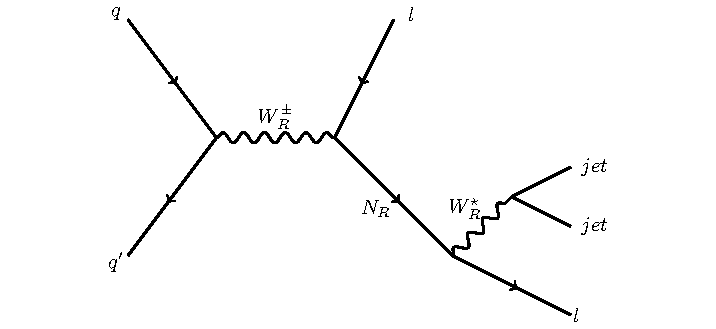
\includegraphics[width=1.0\textwidth]{figures/feynman.pdf}
	\caption{Production of a \WR boson and its decay to two charged leptons and two quarks through 
	a heavy neutrino \nul.}
	\label{fig:wrFeynmanDiagram}
\end{figure}

%%%%%%%%%%%%%%%%%%%%%%%%%%%%%%%%%%%%%%%%%%%%%%%%%%%%%%%%%%%%%%%%%%%%%%%%%%%%%%%%
